%%%%%%%%%%%%%%%%%%%% manuscript.tex %%%%%%%%%%%%%%%%%%%%%%%%%%%%%%%%%%%
%
% Springer proceedings template (svproc class)
% Content: Cold-Start Anomaly Detection for Concrete Surface Crack Inspection
%
%%%%%%%%%%%%%%%% Springer %%%%%%%%%%%%%%%%%%%%%%%%%%%%%%%%%%

\documentclass[runningheads]{llncs}
\usepackage[T1]{fontenc}

\usepackage{graphicx}
\usepackage{caption}
\usepackage{subcaption}
\usepackage{float}
\usepackage{booktabs}
\usepackage{multirow}
\usepackage{array}
\usepackage{xurl}
\usepackage{amssymb}  
\usepackage{amsmath}
\usepackage{makecell}

\usepackage[hidelinks]{hyperref}
\raggedbottom
\setlength{\emergencystretch}{2em}
\begin{document}

\title{Cold-Start Anomaly Detection for Concrete Surface Crack Inspection using PatchCore with Pixel-Level Heatmap Localization}

\titlerunning{Cold-Start Concrete Crack Inspection using PatchCore}

\author{Lam Huynh Khang\inst{1}, Phan Tuan Dat\inst{1}, Nguyen Trong Nhan\inst{1} \and Nguyen Xuan Huy\inst{1}}

\authorrunning{Lam et al.}

\institute{Faculty of Information Technology, FPT University, Ho Chi Minh City, Vietnam\\
\email{khanglhse200666@fpt.edu.vn, ptundatwork@gmail.com, hi.gesar@gmail.com, huynx23@fe.edu.vn}}

\maketitle

\begin{abstract}
Concrete surface cracks are major indicators of structural degradation in civil infrastructure. While supervised deep learning methods achieve high classification accuracy, they depend heavily on extensive labeled defect datasets, which are costly and difficult to obtain in real-world visual inspection. This study reframes concrete crack inspection as a cold-start anomaly detection task, utilizing the PatchCore framework. By training exclusively on crack-free (normal) surface images, the system detects cracks at inference time as deviations from the learned nominal distribution. We systematically evaluate pre-trained ResNet-18 and ResNet-50 backbones under various coreset subsampling ratios (1\%, 5\%, 10\%, 25\%, and 50\%) on the Kaggle Surface Crack Detection dataset. PatchCore achieves a near-perfect image-level Area Under the Receiver Operating Characteristic (AUROC) of 0.9981 and an F1-score of 0.9972 using only 800 training samples. Furthermore, using nearest-neighbor distance mapping, it generates high-resolution anomaly heatmaps that successfully localize crack regions without any pixel-level segmentation training, achieving up to 0.8050 pixel-level AUROC against Canny edge-based pseudo-masks. Our data-efficiency experiments reveal that PatchCore using zero defective training samples outperforms supervised ResNet-50 and EfficientNet-B0 classifiers in low-defect regimes, where the supervised baselines require at least 50 positive training images to reach comparable classification performance. These findings demonstrate that unsupervised cold-start anomaly detection is a highly viable, robust, and data-efficient alternative for civil infrastructure safety monitoring.

\keywords{Concrete crack inspection, Cold-start anomaly detection, PatchCore, Coreset subsampling, Anomaly localization, Data efficiency.}
\end{abstract}

% ---- Introduction ----
\section{Introduction}
\label{sec:introduction}

The inspection of concrete surfaces is a critical component of preventative maintenance and safety monitoring for civil structures, such as bridges, tunnels, roads, and buildings. Concrete cracks represent physical damage resulting from stress, fatigue, environmental conditions, or chemical degradation. Traditional crack inspection relies heavily on manual inspections, which are subjective, labor-intensive, time-consuming, and potentially hazardous. 

With the advent of computer vision and deep learning, automated surface inspection has progressed rapidly. Existing literature heavily treats concrete crack detection as a supervised binary classification problem (crack vs. no-crack) or a supervised semantic segmentation task \cite{Cha2017DeepLC,Golding2022CrackDI,liu2019computer}. Researchers have trained various deep Convolutional Neural Networks (CNNs) like ResNet, VGG, MobileNet, and EfficientNet, or applied object detectors like YOLO and Faster R-CNN on large labeled datasets. While supervised models yield impressive classification and bounding box outcomes, their deployment in industrial and real-world infrastructure faces two fundamental constraints:
First, defective images of cracked concrete are rare in practice compared to the large amount of normal concrete images. Annotating these defects is expensive and works only for specific structures since concrete texture changes depending on the environment. Second, cracks have very different forms such as width, direction, and shape. This makes supervised models overfit to their training images, failing to generalize to new cracks.

To address these challenges, this paper presents a paradigm shift, reframing the problem as \textbf{cold-start visual anomaly detection}. The proposed approach trains a memory-bank-based anomaly detection framework, PatchCore \cite{roth2022towards}, using exclusively normal (crack-free) concrete surface images. During inference, any concrete surface containing cracks is identified as an anomaly because it deviates from the nominal patch feature distribution stored in the memory bank. Additionally, PatchCore naturally generates patch-level anomaly scores, which are upsampled to construct spatial anomaly heatmaps, localizing the crack regions without requiring any pixel-level annotations or bounding box supervisions. 

We conduct a comprehensive evaluation of this framework on the Kaggle Surface Crack Detection dataset \cite{ozgenel2018performance}, referencing other benchmark concrete defect databases such as SDNET2018 \cite{dorafshan2018sdnet2018}. Rather than treating concrete crack detection as a binary classification problem where models require extensive defect examples that are difficult to gather, we reframe the workflow. We first study if PatchCore, an unsupervised memory-bank model originally designed for industrial manufacturing defects, can accurately recognize concrete crack formations having trained only on normal, crack-free surfaces. From this baseline, we explore the model's capacity to localize crack coordinates spatially without any pixel-level segmentation maps, leveraging only nearest-neighbor feature distances. To render the framework practical for deployment on real-world edge devices, we investigate the trade-offs of coreset subsampling ratios (ranging from 1\% to 50\%) on both accuracy and execution speed. Finally, to evaluate the practical advantage of this unsupervised approach, we compare its performance against standard supervised CNN baselines (ResNet-50 and EfficientNet-B0) across varying levels of positive training sample sizes, mapping the data efficiency of cold-start inspection.

The source code for our experiments is publicly available at \url{https://github.com/Welkie/patchcore-concrete-crack-inspection.git}.

\section{Related Work}
\label{sec:related_work}

\subsection{Supervised Concrete Crack Detection}
Computer-vision-based concrete crack detection has transitioned from classical edge-detection methods (such as Sobel and Canny filter configurations) to deep learning. Early work compared deep CNN classifiers to Sobel, Laplacian, and Canny filters, finding that deep features significantly outstrip hand-crafted edge descriptors in handling noisy backgrounds and uneven lighting \cite{dorafshan2018comparison}. Cha et al. \cite{Cha2017DeepLC} pioneered deep-learning-based crack damage detection using CNN architectures, demonstrating high accuracy in complex backgrounds. For pavement and road surfaces, Zhang et al. \cite{zhang2016road} introduced a supervised CNN showing high robustness on road images, and Zhang et al. \cite{Zhang2021RealTime} proposed a real-time detection framework for bridge decks in the frequency domain. 

Özgenel and Sorguç \cite{ozgenel2018performance} compiled the Mendeley "Concrete Crack Images for Classification" dataset and performed comparative training with pretrained architectures like AlexNet, VGG-16, and ResNet, establishing that transfer learning with deep backbones produces excellent image classification results. Comprehensive overviews of these neural classifiers can be found in recent systematic literature reviews \cite{Golding2022CrackDI,Mazni2024Identification}. Beyond classification, researchers have focused on pixel-level semantic crack segmentation. Foundations in this domain rely on U-Net \cite{ronneberger2015u}, which has been adapted to crack configurations, such as U-net fully convolutional networks to segment crack regions accurately \cite{liu2019computer}. However, all these models operate under full supervision, requiring equivalent quantities of positive and negative classes during training.

\subsection{Unsupervised Anomaly Detection and PatchCore}
Unsupervised anomaly detection aims to learn a representation of "normal" data and flag any deviations as anomalies. In computer vision, this has been applied to industrial quality control, pioneered by benchmarks like MVTec AD \cite{bergmann2021mvtec,bergmann2019mvtec}. Early models utilized reconstruction-based approaches (Convolutional Autoencoders, GANs), normalizing flows, or memory-bank-based nearest-neighbors like SPADE \cite{cohen2020sub} and patch distribution models like PaDiM \cite{defard2021padim}. However, reconstruction methods often suffer from "shortcut learning," where anomalous regions are successfully reconstructed, reducing detection sensitivity, while normalizing flows like FastFlow \cite{yu2021fastflow} and knowledge distillation methods like Reverse Distillation \cite{Deng_2022_CVPR} strive to learn robust representations. 

In parallel, within civil engineering and structural health monitoring (SHM), anomaly detection has been investigated to identify damages and sensor abnormalities. Comprehensive reviews of abnormal data detection in SHM outline the transition to unsupervised and deep learning techniques \cite{deng2024abnormal,sonbul2025bridge}. Researchers have proposed vision-based and 1D-CNN frameworks to detect structural changes automatically \cite{bao2019computer,kim2023data}, and more recently, hybrid transformer encoders with 1D-CNN layers have been introduced for time-series and sensor anomaly tracking \cite{nuriev2025data}.

PatchCore, proposed by Roth et al. \cite{roth2022towards}, circumvented general visual anomaly detection limitations by utilizing a memory bank of locally-pooled mid-level patch features extracted from a pre-trained ImageNet backbone. It leverages a greedy coreset selection mechanism to reduce the feature memory footprint while maintaining maximum feature coverage. In industrial benchmarks, PatchCore has achieved state-of-the-art anomaly detection and localization performance. Intel's Anomalib \cite{akcay2022anomalib} has further integrated PatchCore into a generalized library. Despite its success in industrial manufacturing, the feasibility of PatchCore on geological and civil engineering textures, such as concrete crack structures, has not yet been thoroughly explored. This study fills this research gap.

\section{Materials and Methods}
\label{sec:materials_methods}

\subsection{Dataset and Splitting Strategy}
We evaluate the proposed cold-start framework on the Surface Crack Detection dataset hosted on Kaggle \cite{ozgenel2018performance}, which is widely compared with other civil engineering datasets like SDNET2018 \cite{dorafshan2018sdnet2018}. The dataset comprises 4,000 high-resolution RGB images ($227 \times 227$ pixels) divided into 2,000 positive (cracked concrete) and 2,000 negative (normal/crack-free concrete) samples. 

To simulate a realistic cold-start industrial inspection pipeline, we establish an asymmetric splitting strategy. Since unsupervised anomaly detection models train only on normal samples, we split the dataset to match a real-world setup. The training set contains 800 normal images (80\% of all normal images) and does not use any cracked images. The validation set has 100 normal images and 100 cracked images, which helps choose the decision threshold. The final test set consists of 100 normal images and 900 cracked images, which we use to evaluate detection performance and crack localization. This setup mimics actual operations where normal concrete images are easy to collect, but defects are only seen during testing.

\subsection{PatchCore Pipeline Architecture}
The framework uses a pre-trained ImageNet backbone (ResNet-18 or ResNet-50) \cite{he2016deep} without fine-tuning. The operational pipeline consists of three main phases: feature extraction, memory bank construction with coreset selection, and anomaly scoring.

\subsubsection{Feature Extraction and Neighborhood-Aware Patch Pooling}
Given a normal training image $x \in \mathcal{X}_{\text{normal}}$, we feed it through the pre-trained CNN. We extract patch features from intermediate layers, specifically \texttt{layer2} and \texttt{layer3}, which capture mid-level structural features (textures and local geometries) rather than semantic class categories. Let $\phi_l(x)$ represent the feature map output at layer $l \in \{2, 3\}$, which has dimensions $C_l \times H_l \times W_l$. At each spatial coordinate $(h, w)$ where $1 \le h \le H_l$ and $1 \le w \le W_l$, the patch feature is given by the channel vector $f^{(h,w)}_l(x) \in \mathbb{R}^{C_l}$.

To incorporate spatial context, we apply neighborhood-aware patch pooling. For a neighborhood size $p=3$, the pooled feature representation $\mathcal{P}_{h,w}(x)$ at spatial coordinate $(h,w)$ is computed by aggregating features inside a local spatial neighborhood $\mathcal{N}_p(h,w)$:
\begin{equation}
\mathcal{P}_{h,w}(x) = \text{Agg}_{l \in \{2, 3\}} \left( \frac{1}{|\mathcal{N}_p(h,w)|} \sum_{(i,j) \in \mathcal{N}_p(h,w)} f^{(i,j)}_l(x) \right)
\end{equation}
The outputs from layer 2 and layer 3 are bilinearly interpolated to match spatial resolutions, concatenated, and projected using a random linear projection to a fixed dimension $d=512$ to ensure computational efficiency.

\subsubsection{Memory Bank Construction and Greedy Coreset Selection}
By extracting pooled patch features across all coordinates $(h,w)$ for all training images $x \in \mathcal{X}_{\text{normal}}$, we construct a comprehensive memory bank $M$:
\begin{equation}
M = \bigcup_{x \in \mathcal{X}_{\text{normal}}} \left\{ \mathcal{P}_{h,w}(x) \mid h \in [1, H], w \in [1, W] \right\}
\end{equation}
For $N_{\text{train}} = 800$ images, the size of $M$ becomes extremely large (e.g., $800 \times 14 \times 14 = 156,800$ patch vectors). To reduce search latency and memory consumption, we compress $M$ to a coreset subset $M_{\text{sub}} \subset M$ where $|M_{\text{sub}}| \ll |M|$. We solve a minimax facility location optimization problem to find a subset that minimizes the maximum distance between any point in $M$ and its closest counterpart in $M_{\text{sub}}$:
\begin{equation}
M_{\text{sub}} = \text{argmin}_{M' \subset M, |M'| \le c|M|} \max_{x \in M} \min_{y \in M'} \|x - y\|_2
\end{equation}
where $c \in \{0.01, 0.05, 0.10, 0.25, 0.50\}$ is the coreset subsampling ratio. This optimization is solved using a greedy approximation algorithm based on active learning coreset selection \cite{sener2018active}.

\subsubsection{Anomaly Scoring and Localization Heatmap}
At test time, for an input image $x^*$, we extract its patch features $\mathcal{P}(x^*)$. For each patch $y \in \mathcal{P}(x^*)$, we compute its Euclidean distance to the nearest neighbor in $M_{\text{sub}}$. The image-level anomaly score $S(x^*)$ is defined by scaling the maximum patch-level distance:
\begin{equation}
S(x^*) = \left( 1 - \frac{\exp(-\|y^* - z^*\|_2)}{\sum_{z \in \mathcal{N}_b(z^*)} \exp(-\|y^* - z\|_2)} \right) \cdot \|y^* - z^*\|_2
\end{equation}
where $y^* = \text{argmax}_{y \in \mathcal{P}(x^*)} \min_{z \in M_{\text{sub}}} \|y - z\|_2$ is the most anomalous patch, $z^* \in M_{\text{sub}}$ is its nearest neighbor, and $\mathcal{N}_b(z^*)$ is the set of $b=9$ nearest neighbors of $z^*$ in $M_{\text{sub}}$.

To compute the pixel-level anomaly localization heatmap, we assign each patch coordinate $(h,w)$ of the test image its individual anomaly distance $s(h,w) = \min_{z \in M_{\text{sub}}} \|\mathcal{P}_{h,w}(x^*) - z\|_2$. The low-resolution map of size $H_{\text{map}} \times W_{\text{map}}$ is upsampled back to the original image dimensions $H \times W$ using bilinear interpolation and smoothed using a Gaussian filter:
\begin{equation}
S_{\text{pixel}}(x^*) = G_{\sigma} * \text{Upsample}\left( [s(h,w)]_{H_{\text{map}} \times W_{\text{map}}} \right)
\end{equation}
where $G_{\sigma}$ is a Gaussian smoothing kernel with $\sigma=4$.

\subsection{Evaluation of Pixel-Level AUROC via Pseudo-Ground-Truth Masks}
The Kaggle Surface Crack Detection dataset only provides image-level binary labels (crack/no-crack) and lacks pixel-level annotations (ground-truth masks). To quantitatively evaluate the pixel-level localization performance, we automatically generate a set of pseudo-ground-truth masks for the test images. For each positive image, we process it in three steps. First, we convert the image to grayscale and apply a $5 \times 5$ Gaussian blur to remove surface noise. Second, we run Canny edge detection with thresholds set at 30 and 100 to find the boundaries of the cracks. Third, we apply morphological dilation with a $3 \times 3$ rectangular kernel for one iteration to connect the gaps in the edges and form a continuous shape. This generates binary masks where the crack body is marked as 1 and the intact concrete is 0.

\section{Experimental Results}
\label{sec:results}

\subsection{Experimental Configuration}
All experiments are implemented in PyTorch and run on a single NVIDIA T4 GPU. Feature similarity searches are executed using the FAISS library to ensure high-speed nearest-neighbor computations. The input images are resized to $256 \times 256$ pixels and center-cropped to $224 \times 224$ pixels. 

\subsection{Coreset Subsampling Ablation and Execution Latency}
We first analyze the baseline detection capability of PatchCore along with the impact of coreset subsampling ratios $\lambda \in \{1\%, 5\%, 10\%, 25\%, 50\%\}$ using ResNet-18 and ResNet-50 backbones. The results are summarized in Table~\ref{tab:patchcore_ablation}.

\begin{table}[H]
\centering
\caption{PatchCore coreset ablation results on the Concrete Surface Crack dataset showing detection performance and resource metrics.}
\label{tab:patchcore_ablation}
\resizebox{\textwidth}{!}{%
\begin{tabular}{lcccccccc}
\toprule
\textbf{Backbone} & \makecell{\textbf{Coreset}\\\textbf{Ratio}} & \makecell{\textbf{Image}\\\textbf{AUROC}} & \makecell{\textbf{Pixel}\\\textbf{AUROC}} & \makecell{\textbf{Image}\\\textbf{F1-Score}} & \makecell{\textbf{Fitting}\\\textbf{Time (s)}} & \makecell{\textbf{Latency}\\\textbf{(ms/img)}} & \makecell{\textbf{Memory}\\\textbf{Points}} & \makecell{\textbf{Memory}\\\textbf{Size (MB)}} \\
\midrule
\multirow{5}{*}{ResNet-18} 
 & 1\%  & 0.9969 & 0.7997 & 0.9945 & 53.84  & 31.37  & 6,272   & 12.25  \\
 & 5\%  & 0.9980 & 0.8011 & 0.9956 & 196.47 & 35.73  & 31,360  & 61.25  \\
 & 10\% & 0.9979 & 0.8027 & 0.9956 & 376.05 & 41.08  & 62,720  & 122.50 \\
 & 25\% & 0.9978 & 0.8050 & 0.9956 & 907.82 & 66.88  & 156,800 & 306.25 \\
 & 50\% & 0.9974 & 0.8050 & 0.9950 & 1790.89& 110.64 & 313,600 & 612.50 \\
\midrule
\multirow{5}{*}{ResNet-50} 
 & 1\%  & 0.9973 & 0.7827 & 0.9967 & 61.49  & 34.35  & 6,272   & 12.25  \\
 & 5\%  & 0.9968 & 0.7856 & 0.9972 & 202.21 & 39.83  & 31,360  & 61.25  \\
 & 10\% & 0.9976 & 0.7864 & 0.9972 & 379.12 & 47.15  & 62,720  & 122.50 \\
 & 25\% & 0.9980 & 0.7865 & 0.9972 & 909.27 & 73.48  & 156,800 & 306.25 \\
 & 50\% & 0.9981 & 0.7865 & 0.9972 & 1791.23& 118.11 & 313,600 & 612.50 \\
\bottomrule
\end{tabular}%
}
\end{table}

The experimental data demonstrates that PatchCore achieves a near-perfect image-level AUROC of over 0.996 across all ratios and backbones. The highest image-level AUROC of 0.9981 is achieved using ResNet-50 at a 50\% coreset ratio, while ResNet-18 achieves a peak image-level AUROC of 0.9980 at a 5\% ratio. Furthermore, compressing the memory bank using coreset sampling dramatically reduces inference latency and memory size with negligible impact on detection accuracy. For instance, reducing the coreset ratio of ResNet-18 from 50\% to 10\% reduces the memory index size from 612.50 MB to 122.50 MB and speeds up inference from 110.64 ms/image to 41.08 ms/image, while the pixel localization AUROC only shifts from 0.8050 to 0.8027.

\subsection{Comparison with Supervised Classification under Data Scarcity}
To evaluate how the cold-start paradigm compares with standard supervised models in resource-limited scenarios, we train ResNet-50 \cite{he2016deep} and EfficientNet-B0 \cite{tan2019efficientnet} classifiers under a fully supervised paradigm. The models are trained for 10 epochs using Adam optimizer ($\text{LR}=10^{-4}$, batch size 16). We vary the availability of labeled cracked images during training ($N_{\text{pos}} \in \{5, 10, 50, 100, 200\}$) while keeping 1,600 normal images to evaluate data efficiency. The baseline testing results are presented in Table~\ref{tab:supervised_baselines}.

\begin{table}[H]
\centering
\caption{Supervised baseline classification results under varying positive training sample sizes for data efficiency comparison.}
\label{tab:supervised_baselines}
\resizebox{\textwidth}{!}{%
\begin{tabular}{lcccccc}
\toprule
\textbf{Model} & \makecell{\textbf{Num Training}\\\textbf{Positives}} & \textbf{Accuracy} & \textbf{AUROC} & \textbf{F1-Score} & \textbf{Precision} & \textbf{Recall} \\
\midrule
\multirow{5}{*}{ResNet-50} 
 & 5   & 0.4490 & 0.9064 & 0.5588 & 1.0000 & 0.3878 \\
 & 10  & 0.3180 & 0.8522 & 0.3900 & 1.0000 & 0.2422 \\
 & 50  & 0.9710 & 1.0000 & 0.9836 & 1.0000 & 0.9678 \\
 & 100 & 0.9820 & 1.0000 & 0.9899 & 1.0000 & 0.9800 \\
 & 200 & 0.9610 & 0.9983 & 0.9779 & 1.0000 & 0.9567 \\
\midrule
\multirow{5}{*}{EfficientNet-B0} 
 & 5   & 0.2240 & 0.9515 & 0.2422 & 1.0000 & 0.1378 \\
 & 10  & 0.3490 & 0.9049 & 0.4334 & 1.0000 & 0.2767 \\
 & 50  & 0.9610 & 0.9995 & 0.9779 & 1.0000 & 0.9567 \\
 & 100 & 0.9660 & 1.0000 & 0.9807 & 1.0000 & 0.9622 \\
 & 200 & 0.9540 & 0.9999 & 0.9738 & 1.0000 & 0.9489 \\
\bottomrule
\end{tabular}%
}
\end{table}

The comparative results indicate that supervised classifiers are highly sensitive to class imbalance and data scarcity. With fewer than 10 positive training samples, the supervised models fail to generalize, yielding F1-scores as low as 0.2422 due to extreme recall failures. The supervised models require at least 50 positive training images to match the F1 performance that unsupervised PatchCore achieves with **zero** positive training samples.

\section{Discussion}
\label{sec:discussion}

\subsection{Unsupervised Crack Detection and Localization Analysis}
Unsupervised anomaly detection has historically been viewed as a harder problem than supervised classification because the network is never exposed to defect examples. However, our findings reveal that PatchCore achieves outstanding performance on concrete cracks (Image AUROC > 0.997). This high accuracy is because concrete cracks introduce a sharp disruption in local texture. Intact concrete consists of homogeneous, semi-periodic rough textures. When a crack is present, it forms a dark, linear geometric anomaly that behaves as a clear out-of-distribution patch compared to normal concrete patches.

Furthermore, we evaluate the spatial localization capacity. ResNet-18 achieves a pixel-level AUROC of 0.8050, outperforming ResNet-50 which scores 0.7865. This result suggests that the feature representation of ResNet-18 contains finer spatial detail, while ResNet-50 layer activations are more semantically compressed, slightly blurring the local patch boundary.

\subsection{Inference Speed vs. Data Efficiency Trade-Off}
To visualize the performance behaviors, we refer to the curves generated in our experiments.

\begin{figure}[H]
    \centering
    \begin{subfigure}[b]{0.48\textwidth}
        \centering
        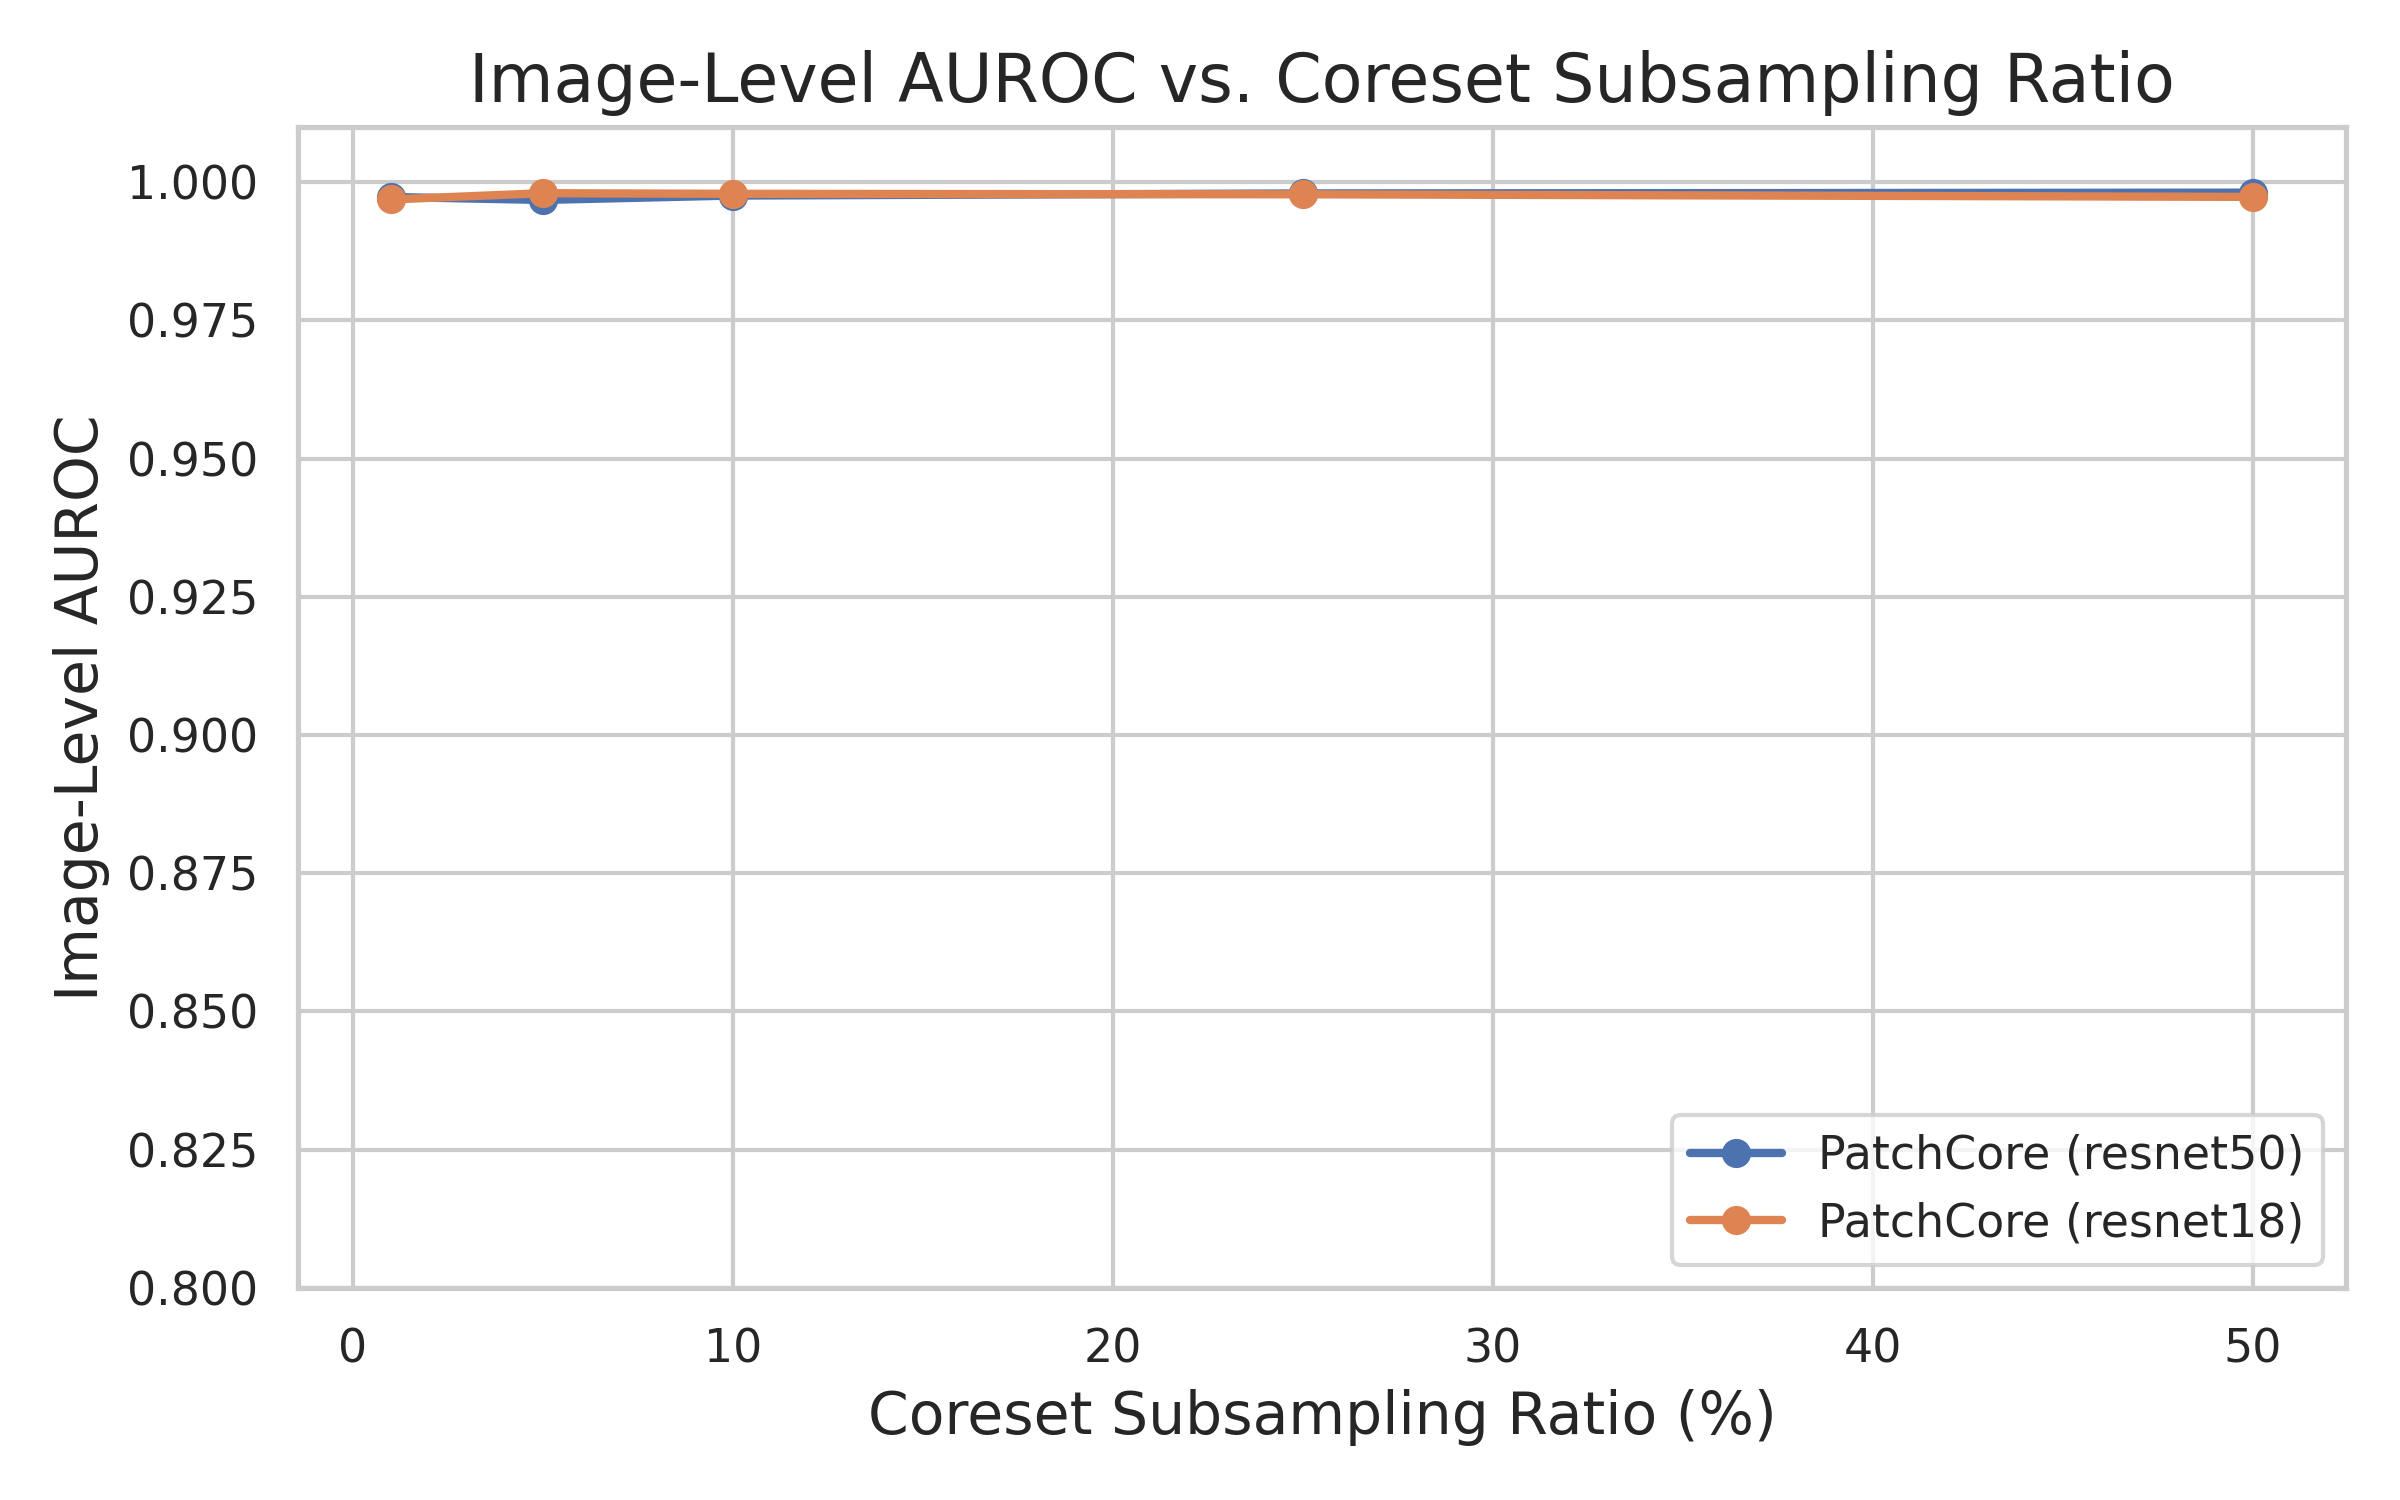
\includegraphics[width=\textwidth]{results/plot_auroc_vs_coreset.png}
        \caption{Image AUROC vs. Coreset Ratio}
        \label{fig:auroc_vs_coreset}
    \end{subfigure}
    \hfill
    \begin{subfigure}[b]{0.48\textwidth}
        \centering
        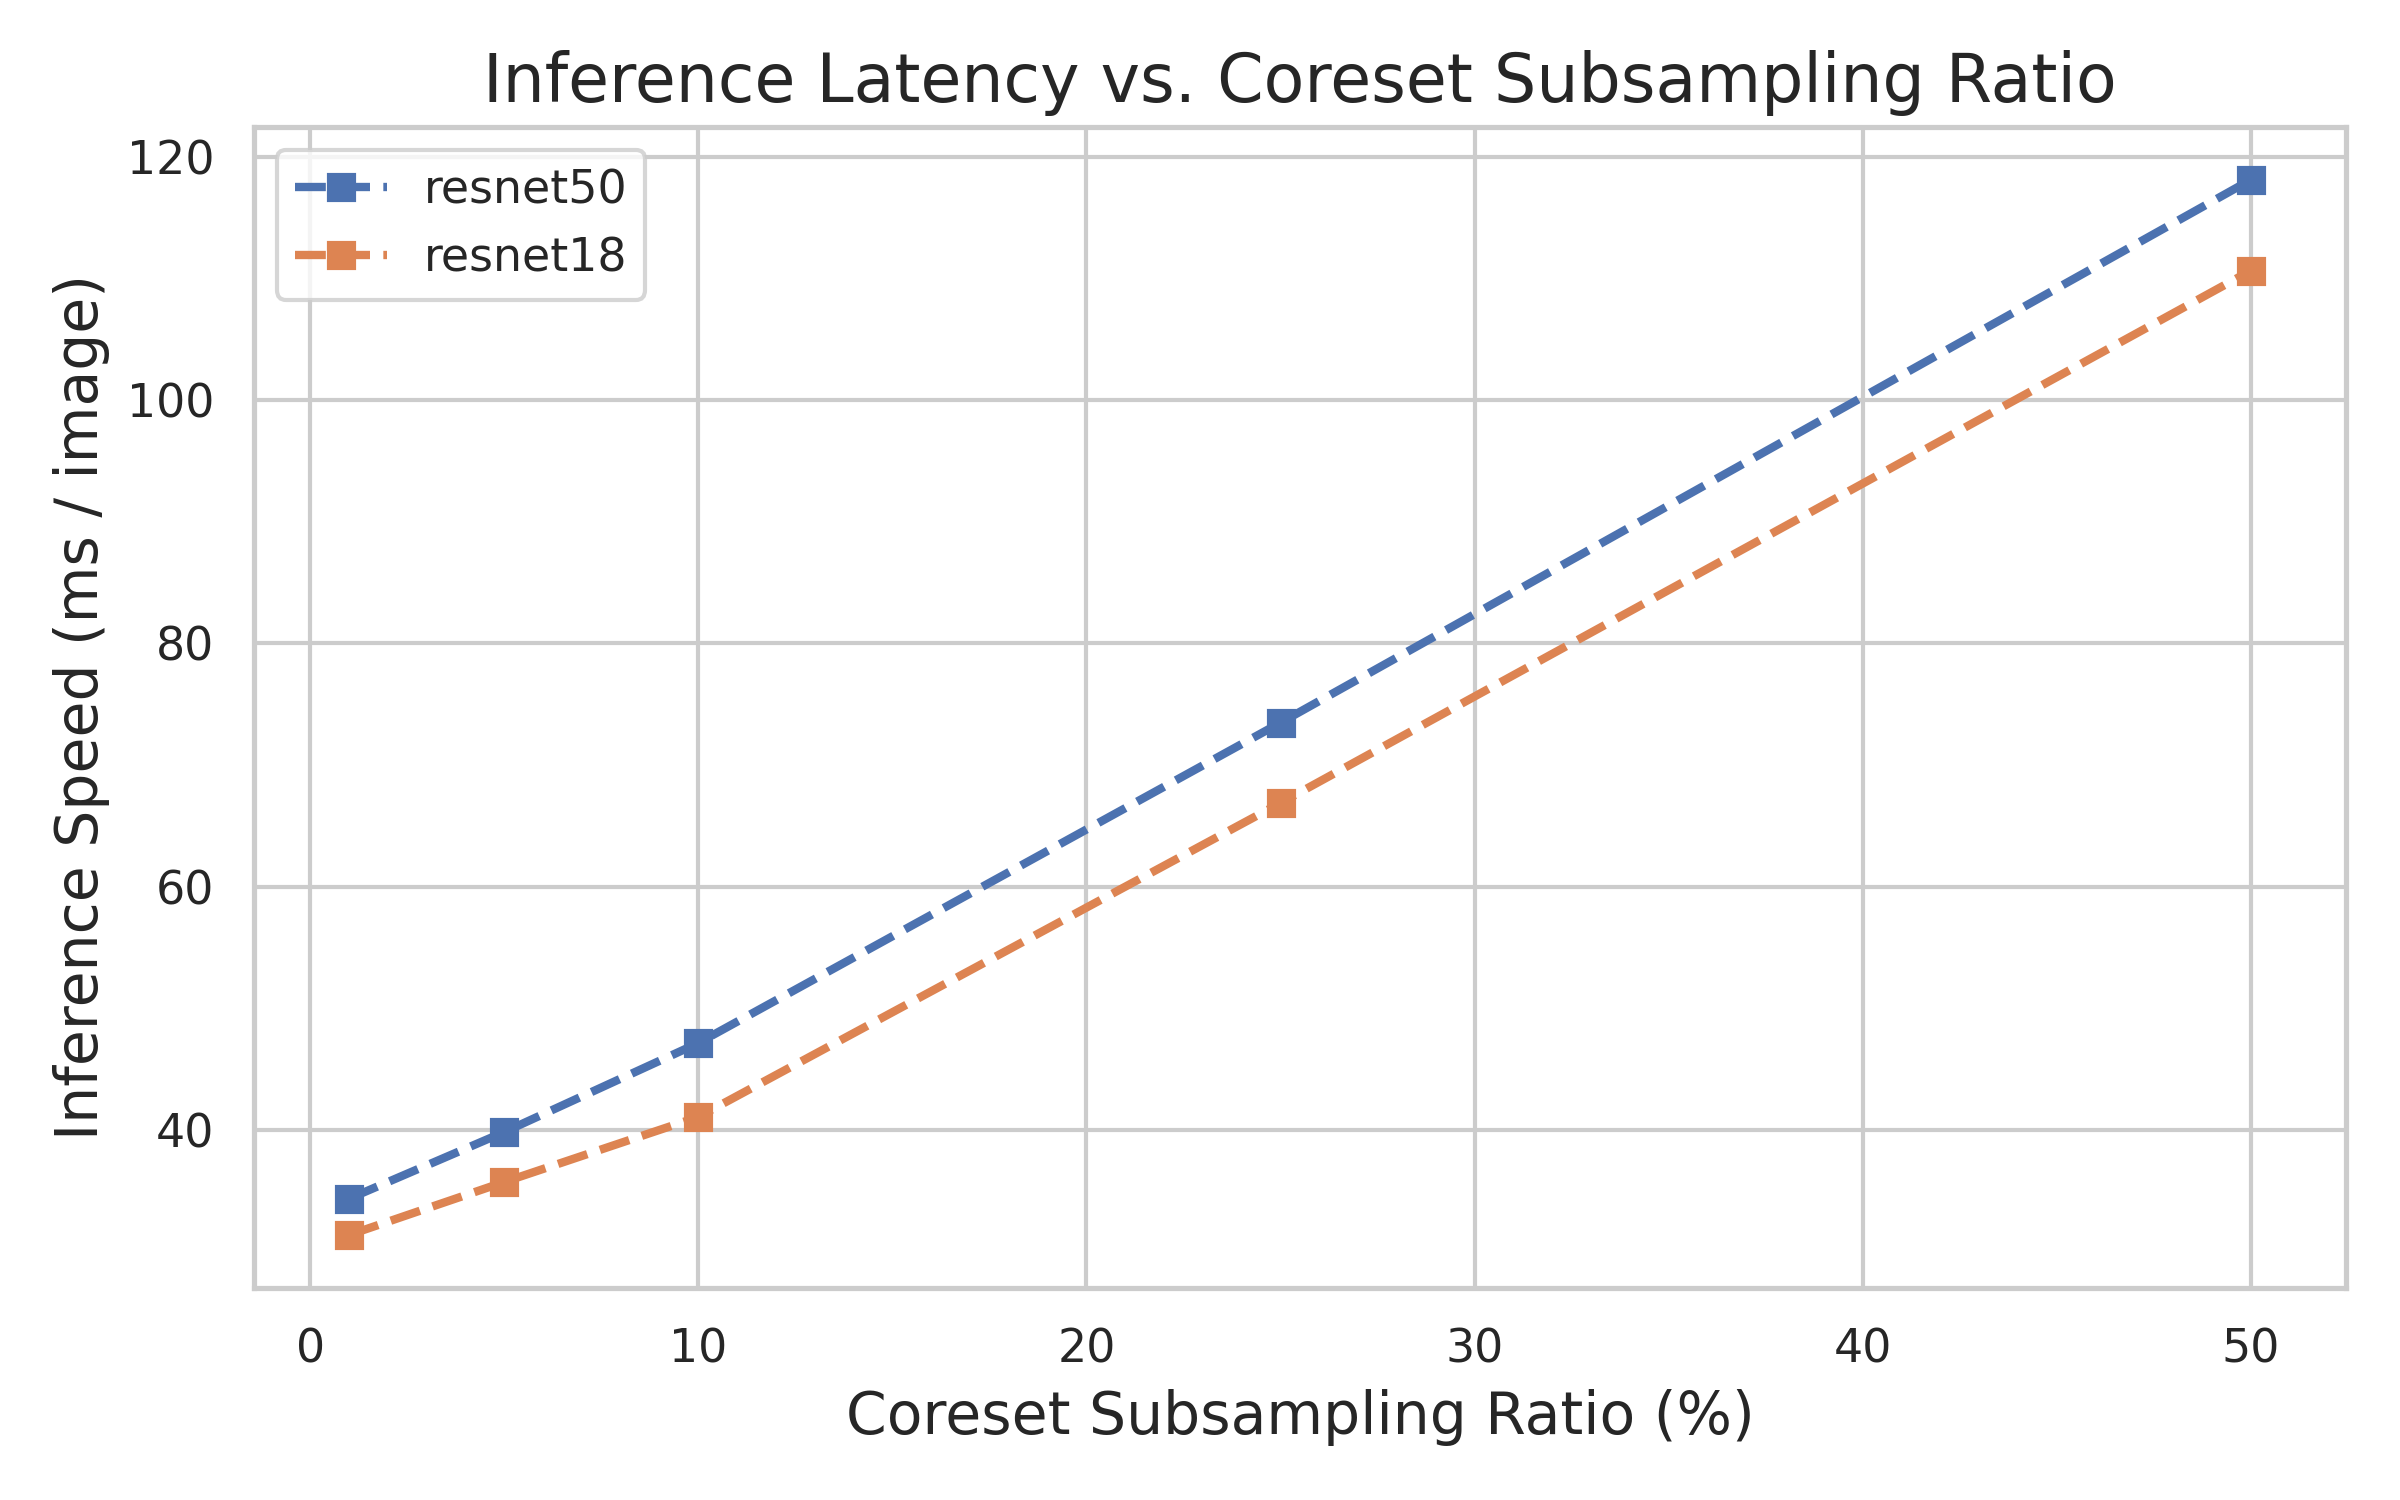
\includegraphics[width=\textwidth]{results/plot_latency_vs_coreset.png}
        \caption{Inference Latency vs. Coreset Ratio}
        \label{fig:latency_vs_coreset}
    \end{subfigure}
    \caption{Analysis of Coreset Subsampling Ratio Trade-off between accuracy and speed.}
    \label{fig:coreset_tradeoff}
\end{figure}

Fig.~\ref{fig:coreset_tradeoff} illustrates the impact of the coreset ratio. While the image-level AUROC remains stable above 0.996 across all ratios (Fig.~\ref{fig:auroc_vs_coreset}), the inference latency (Fig.~\ref{fig:latency_vs_coreset}) grows linearly. A 10\% coreset ratio provides the optimal trade-off point: it achieves virtually the same detection and localization metrics as the 50\% ratio, but reduces inference time by 60\% and memory size to only 122.50 MB.

\begin{figure}[H]
    \centering
    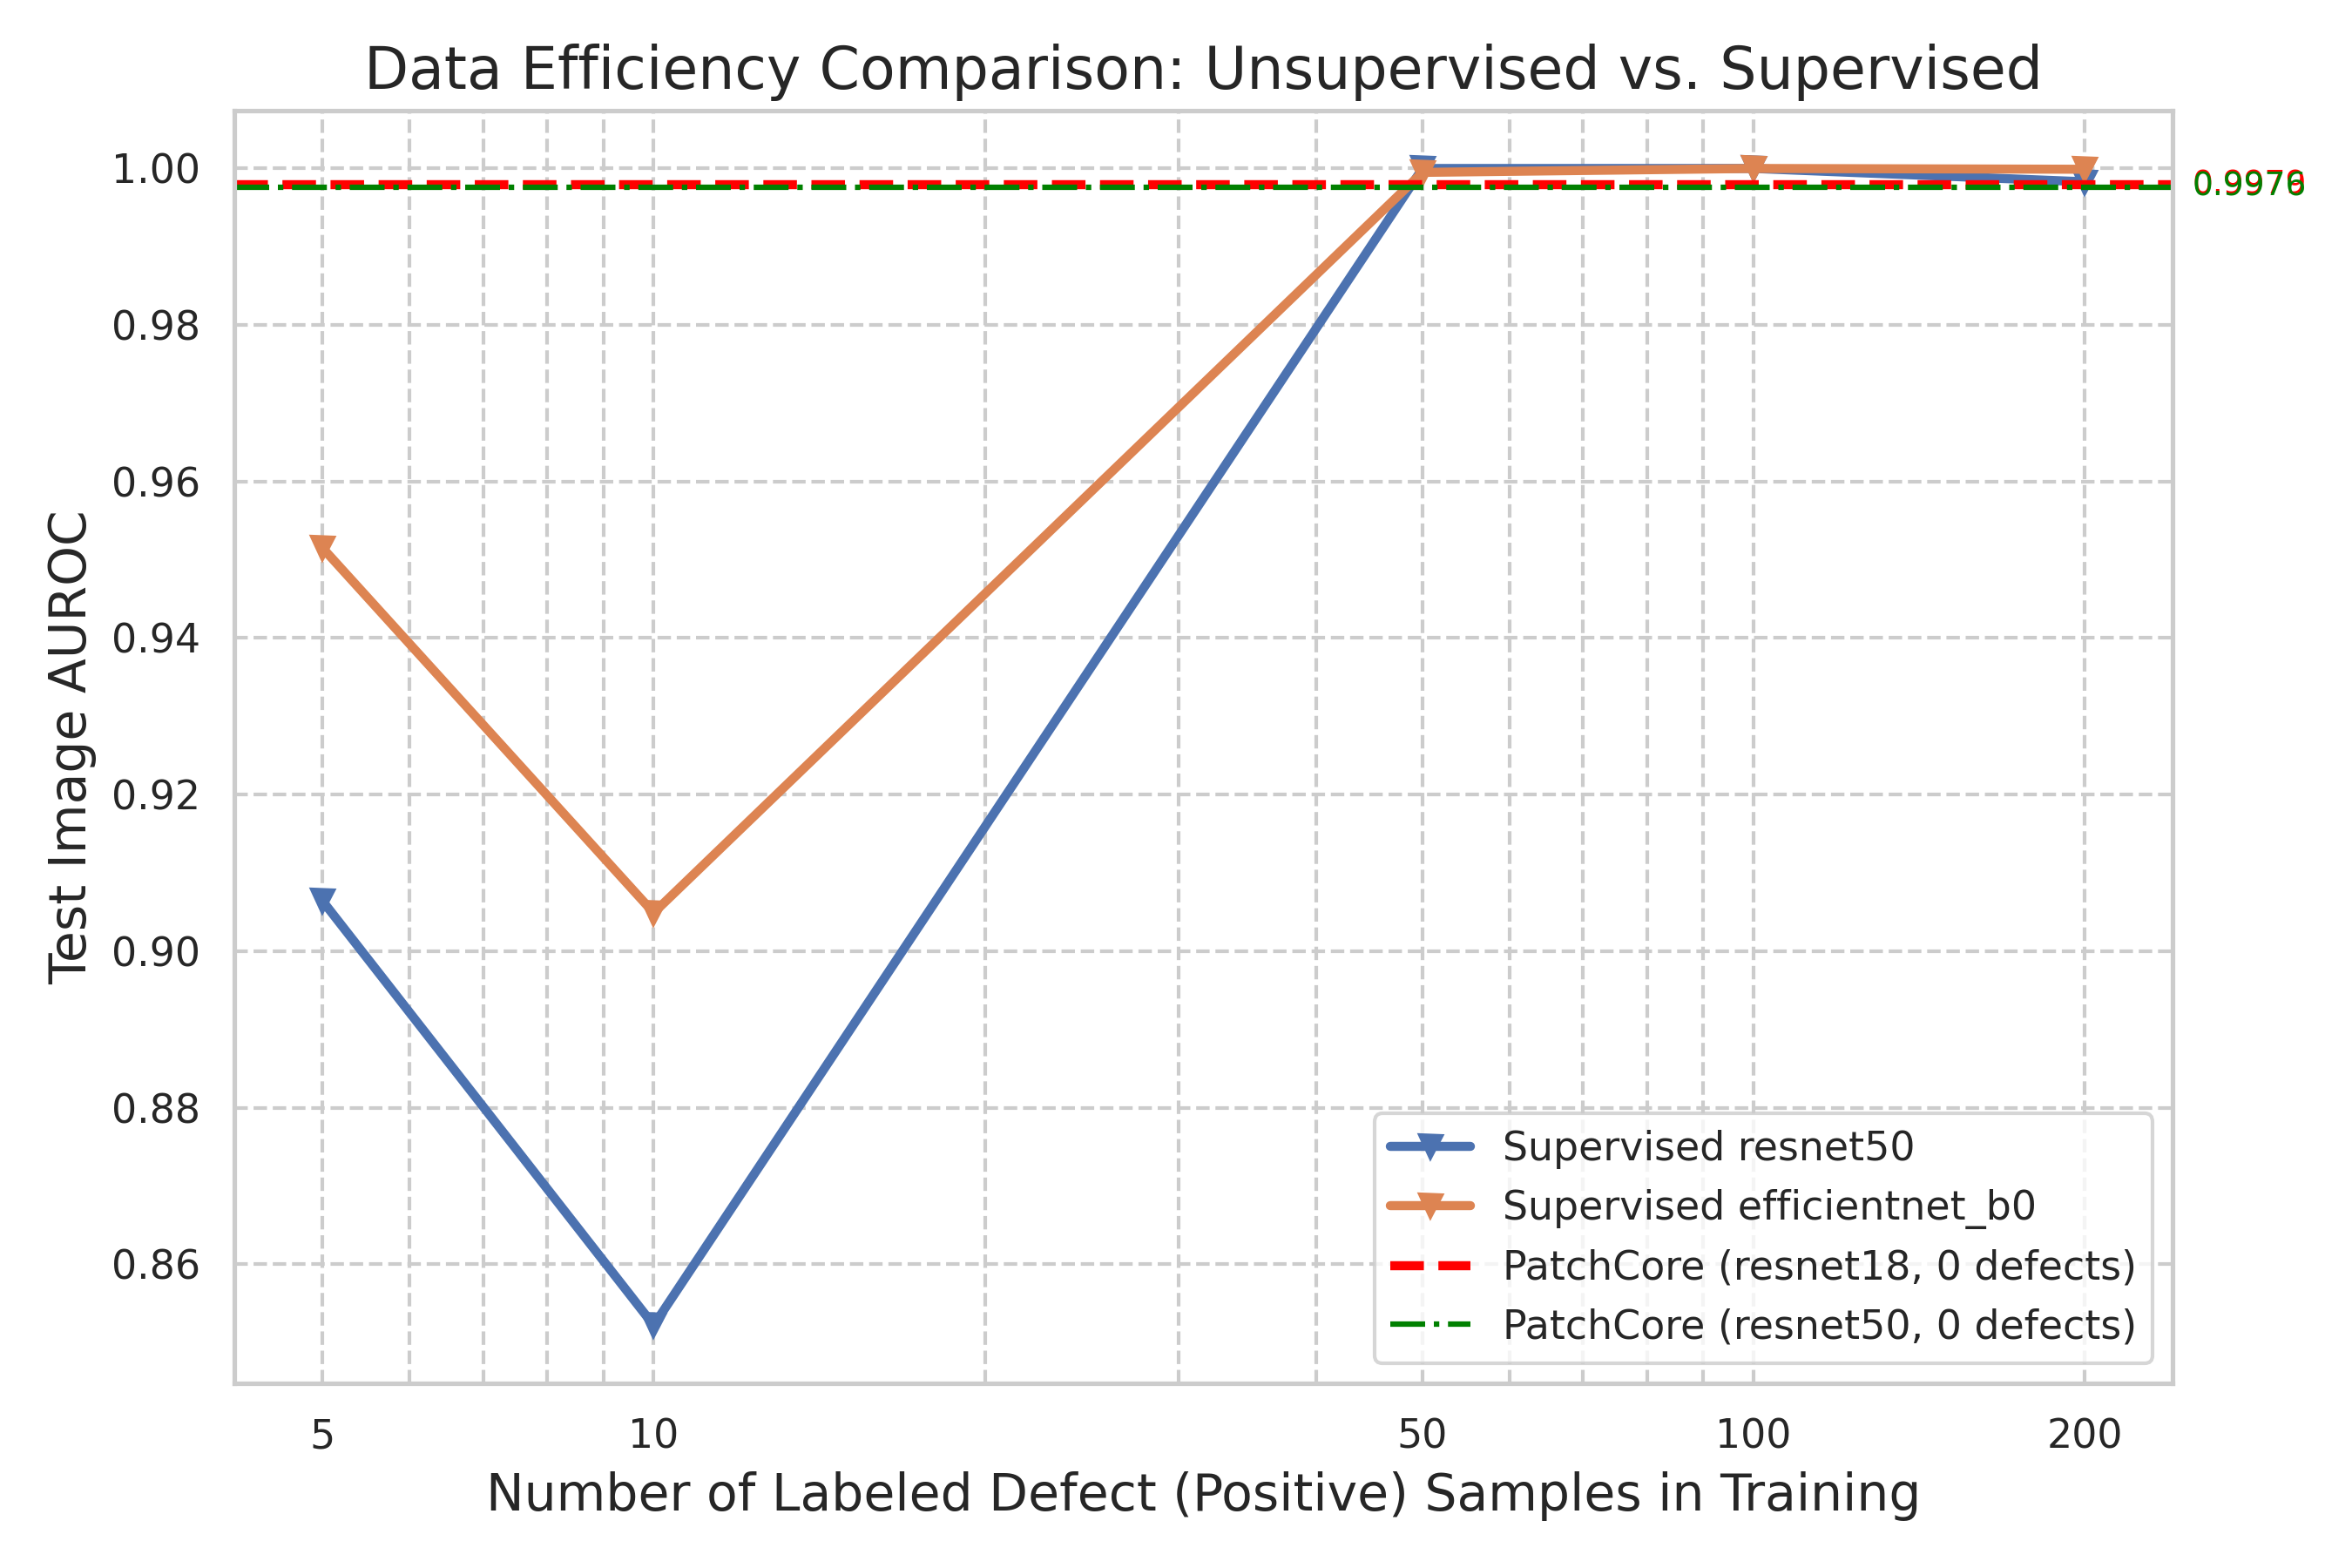
\includegraphics[width=0.8\textwidth]{results/plot_data_efficiency.png}
    \caption{Data Efficiency Comparison: Unsupervised PatchCore vs. Supervised CNNs.}
    \label{fig:data_efficiency}
\end{figure}

Fig.~\ref{fig:data_efficiency} highlights the data efficiency curves. The horizontal lines represent unsupervised PatchCore models trained with zero cracked samples. When supervised models have access to only 5 to 10 positive samples, they perform significantly worse. This demonstrates that in "cold-start" environments where defects are unavailable or extremely rare, unsupervised PatchCore is a far more robust choice.

\subsection{Qualitative Visualization and Local Anomaly Heatmaps}
To visually inspect the localization quality, we examine the qualitative crack heatmap overlays for ResNet-18 (Fig.~\ref{fig:localization_resnet18}) and ResNet-50 (Fig.~\ref{fig:localization_resnet50}).

\begin{figure}[H]
    \centering
    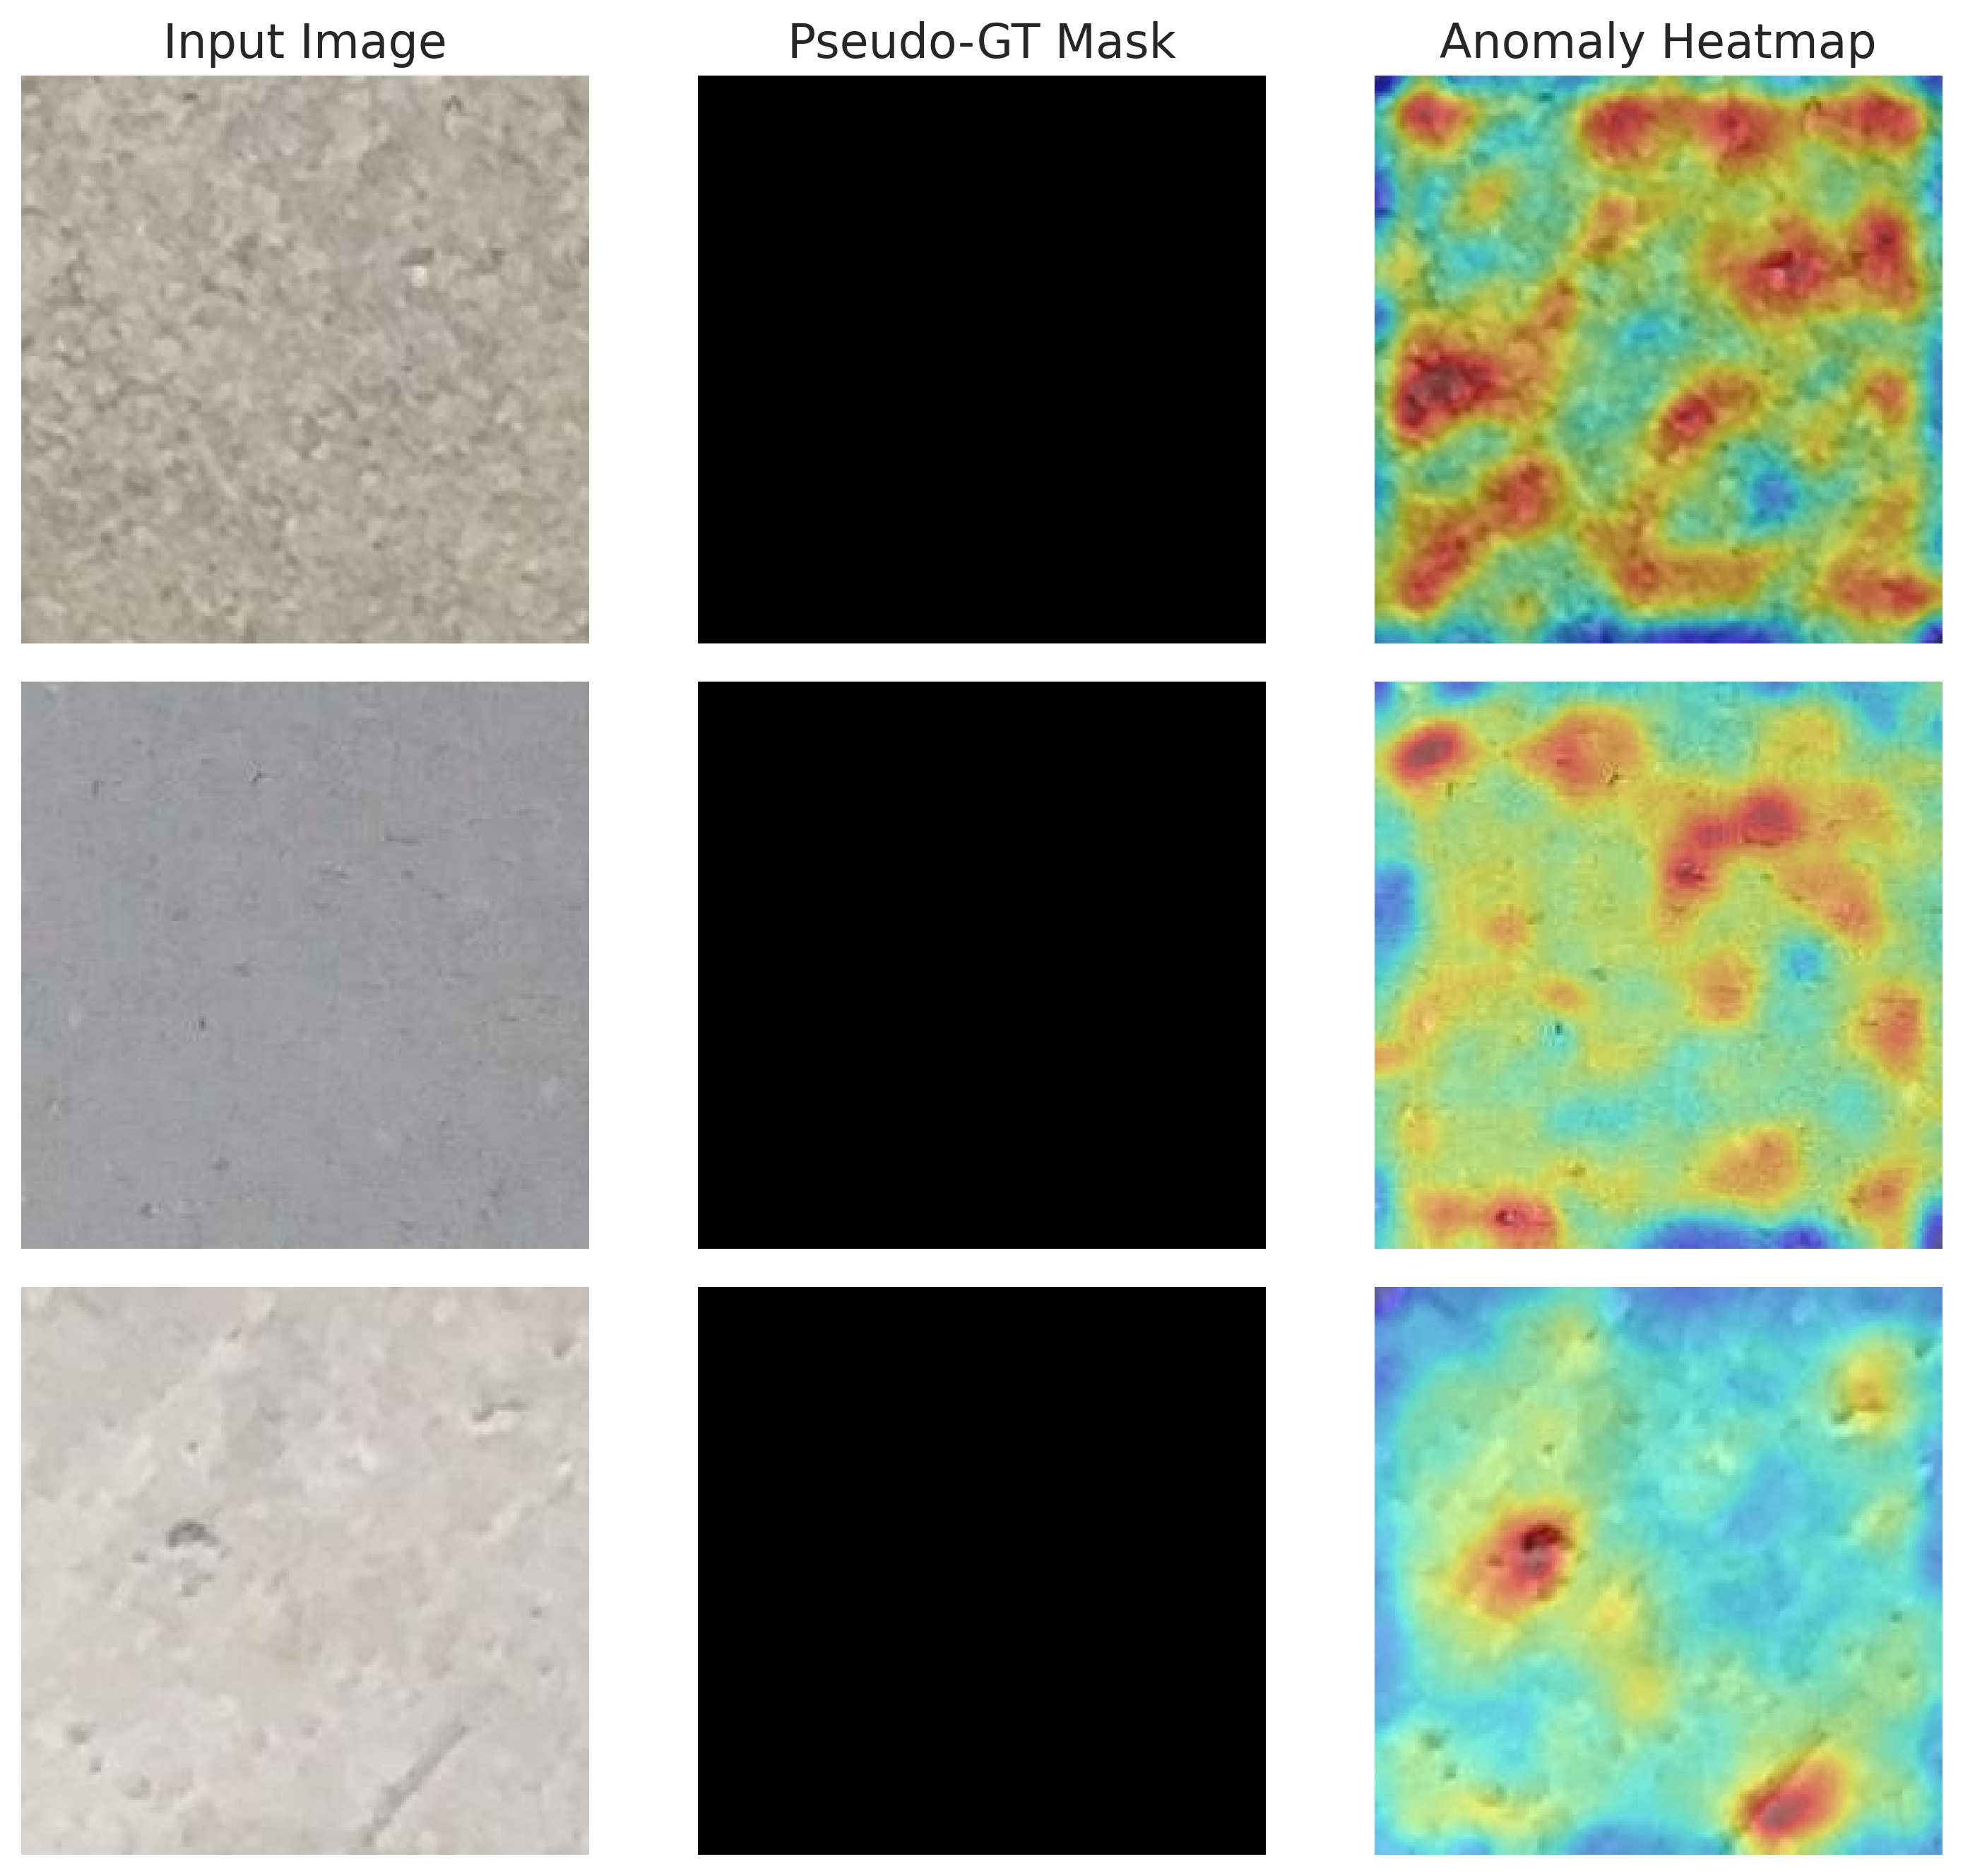
\includegraphics[width=0.95\textwidth]{results/visual_localization_resnet18.png}
    \caption{Qualitative Crack Heatmap Overlays (ResNet-18, 10\% Coreset).}
    \label{fig:localization_resnet18}
\end{figure}

\begin{figure}[H]
    \centering
    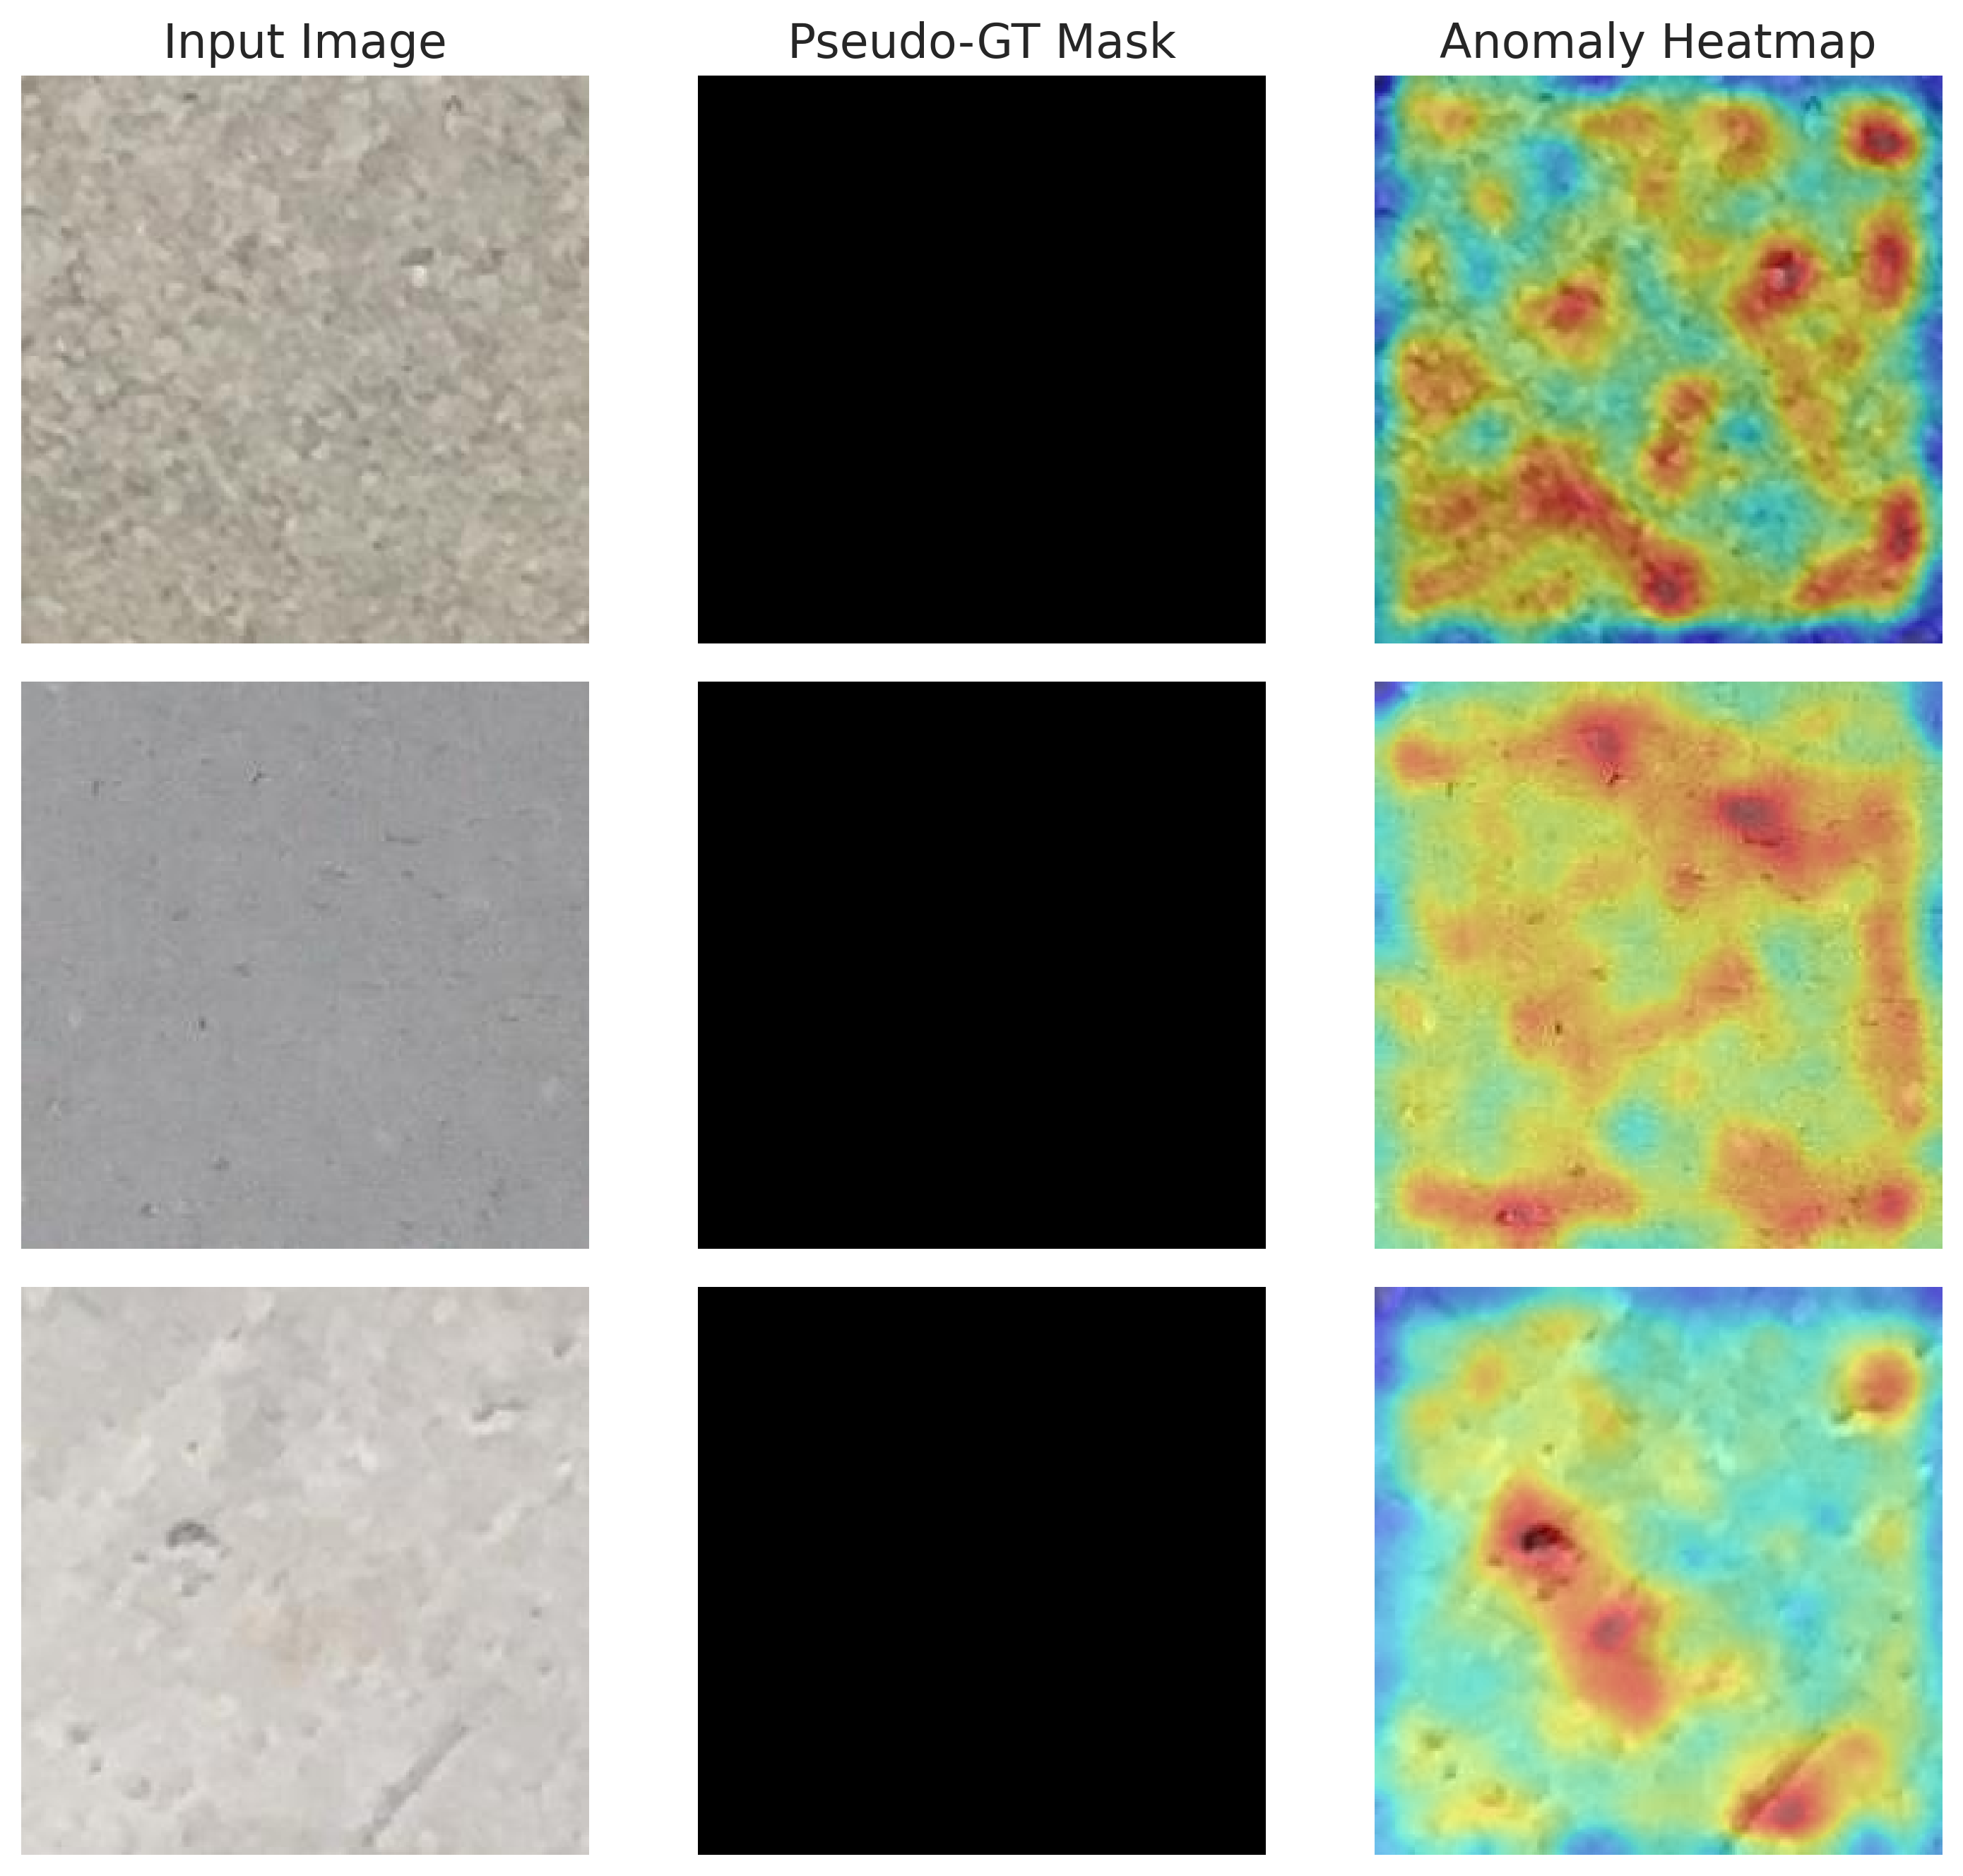
\includegraphics[width=0.95\textwidth]{results/visual_localization_resnet50.png}
    \caption{Qualitative Crack Heatmap Overlays (ResNet-50, 10\% Coreset).}
    \label{fig:localization_resnet50}
\end{figure}

As shown in Fig.~\ref{fig:localization_resnet18} and Fig.~\ref{fig:localization_resnet50}, the generated anomaly heatmaps successfully trace the physical shape and location of the cracks. The heatmaps display strong peak values precisely along the crack trajectories, with zero or minimal background activation on the normal concrete areas. This localization is achieved without any pixel-level supervision or bounding box annotations during training.

\subsection{Research Limitations and Future Prospects}
While PatchCore achieves excellent performance, some limitations remain:
First, PatchCore assumes that normal samples have a similar texture. If a concrete structure has very different surface patterns, joint lines, or markings, it can cause false alarms. Second, we evaluate pixel performance using masks made with Canny edge detection. Although these masks show the crack shapes well, they can have noise. Future studies should use human-annotated masks to test the heatmaps more accurately.

\section{Conclusion and Future Work}
\label{sec:conclusion}

In this paper, we reframed the concrete surface crack inspection problem as cold-start visual anomaly detection, implementing the PatchCore framework. Training exclusively on 800 normal concrete surface images, PatchCore achieves a near-perfect image-level AUROC of 0.9981 and an F1-score of 0.9972, without requiring any cracked images during training. Furthermore, the framework generates high-quality anomaly heatmaps that accurately localize crack trajectories without any pixel-level supervision, achieving up to 0.8050 pixel-level AUROC. Our comparative analysis confirms that PatchCore drastically outperforms supervised classifiers in low-defect regimes, where supervised baselines require at least 50 positive training images to match PatchCore's zero-shot defect classification performance. Additionally, we demonstrated that a 10\% coreset subsampling ratio provides the optimal trade-off, cutting inference latency by 60\% and memory size by 80\% with no loss in accuracy.

Future research will focus on extending the memory bank representation to handle heterogeneous concrete surfaces with multiple textures, integrating temporal tracking to monitor crack growth, and evaluating the framework on real-world mobile edge devices.

\section*{Declaration of competing interest}
Declaration of generative AI and AI-assisted technologies in the writing process: ChatGPT was used for assisting with language editing only. The authors reviewed and revised the manuscript and take full responsibility for the accuracy and integrity of the work.

% ---- Bibliography ----
\bibliographystyle{splncs03_unsrt}
\bibliography{references}

\end{document}